As discussed in Section \ref{methodsec:fourier}, a naive DFT implementation has a runtime of $\mathcal{O}(N^2)$ for an input signal $x=\{x_0,\dots,x_{N-1}\}$. The Fast Fourier Transform (FFT) significantly speeds up this process. The name ``FFT" actually refers to a whole family of algorithms that can solve a wider range of problems, but all of them take advantage of the symmetry in the complex plane to use a divide and conquer scheme. The FFT was first formally proposed by Cooley and Tukey in their 1965 paper \cite{CooleyTukey}, and the mathematical discussion here is inspired by Broughton \cite{broughton2009discrete}. We start with Equation \ref{eq:dfttransform} for the DFT Transform, but instead write it as 
\begin{equation}
    X_{(N/2)k_1+k_0}=\sum_{m=0}^{N-1}x_m(-1)^{k_1m}e^{-2\pi ik_0/N},\label{eq:fftstart}
\end{equation}
where $k_1\in\{0,1\}$ and $0\leq k_2<N/2$. Note that now when $k_1=0$ we are referring to the first $N/2$ coefficients, while when $k_1=1$ we are referring to the second half. If we then split the sum into its even and odd terms and simplify, we get that 
\begin{equation}
    X_{k_0}=F_1(k_0)+e^{-2\pi ik_0/N}F_2(k_0)\label{eq:fftrelation1}
\end{equation}
and
\begin{equation}
    X_{N/2+k_0}=F_1(k_0)-e^{-2\pi ik_0/N}F_2(k_0),\label{eq:fftrelation2}
\end{equation}
where 
\begin{equation}
    F_1(k_0)=\sum_{m=0}^{N-1}x_{2m}e^{-2\pi ik_0/(N/2)}\label{eq:evenfft}
\end{equation}
and 
\begin{equation}
    F_2(k_0)=\sum_{m=0}^{N-1}x_{2m+1}e^{-2\pi ik_0/(N/2)}.\label{eq:oddfft}
\end{equation}
Note that $F_1(k_0)$ and $F_2(k_0)$ describe the DFT on the even and odd terms of the original signal $x$, respectively. In other words, to get the full length $N$ DFT, one needs only to calculate the length $N/2$ DFT on the even and odd terms, then sum them to get the first $N/2$ terms for the full DFT (Eq. \ref{eq:fftrelation1}) and take their difference for the second $N/2$ terms (Eq. \ref{eq:fftrelation2}). This process can then be repeated recursively, further breaking down each half transform. The first step of this process is shown in Fig. \ref{fig:FFTalgorithm}. In this sense, the FFT is a classic divide and conquer algorithm, and an application of the Master Theorem can rigorously prove the $\mathcal{O}(N\log N)$ runtime that results. We refer a reader interested in the derivations of the relations in Equation \ref{eq:fftrelation1} and Equation \ref{eq:fftrelation2} once again to Broughton \cite{broughton2009discrete}. For an in-depth walkthrough of how the FFT can be implemented efficiently, see the CP algorithms page \cite{CPAFFT}.

\begin{figure}[ht]
    \centering
    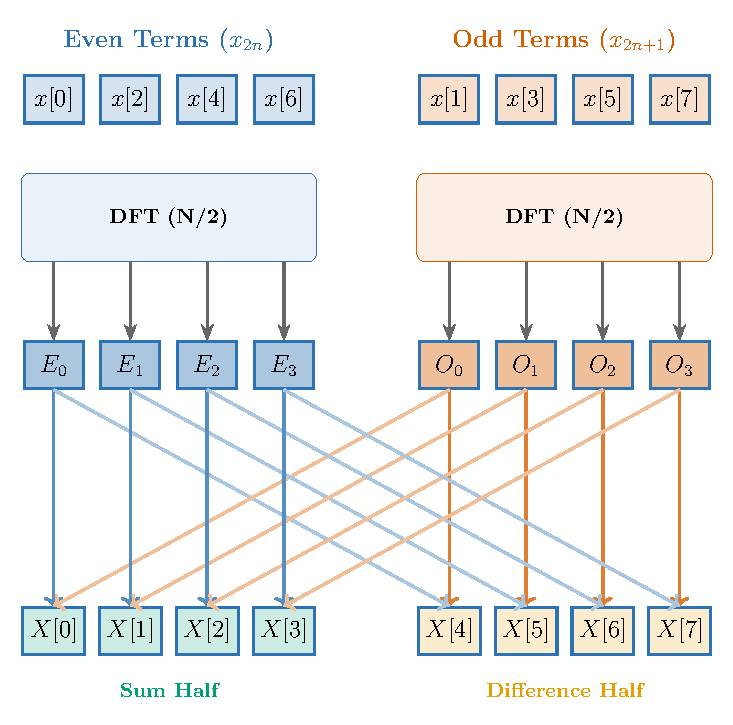
\includegraphics[width=1\linewidth]{methods/Fourierdiagrams/fft.pdf}
    \caption{The first recursive step in the FFT.}
    \label{fig:FFTalgorithm}
\end{figure}
